\documentclass[10pt]{article}
\usepackage{graphicx}
\graphicspath{ {/home/ayush/school/AoA/hw5} }
\usepackage{mathtools}
\usepackage[margin=1.25in]{geometry}
\newcommand{\tab}[1]{\hspace{.05\textwidth}\rlap{#1}}
\begin{document}
\vspace*{\fill}
\begin{Huge}
\begin{center}
HW5\\
Name: Ayush Jain\\
UNI: aj2672
\end{center}
\end{Huge}
\vspace*{\fill}
\newpage
\section{Problem 1}
\textbf{Exercise 22.2-6}\\
\begin{figure}[ht!]
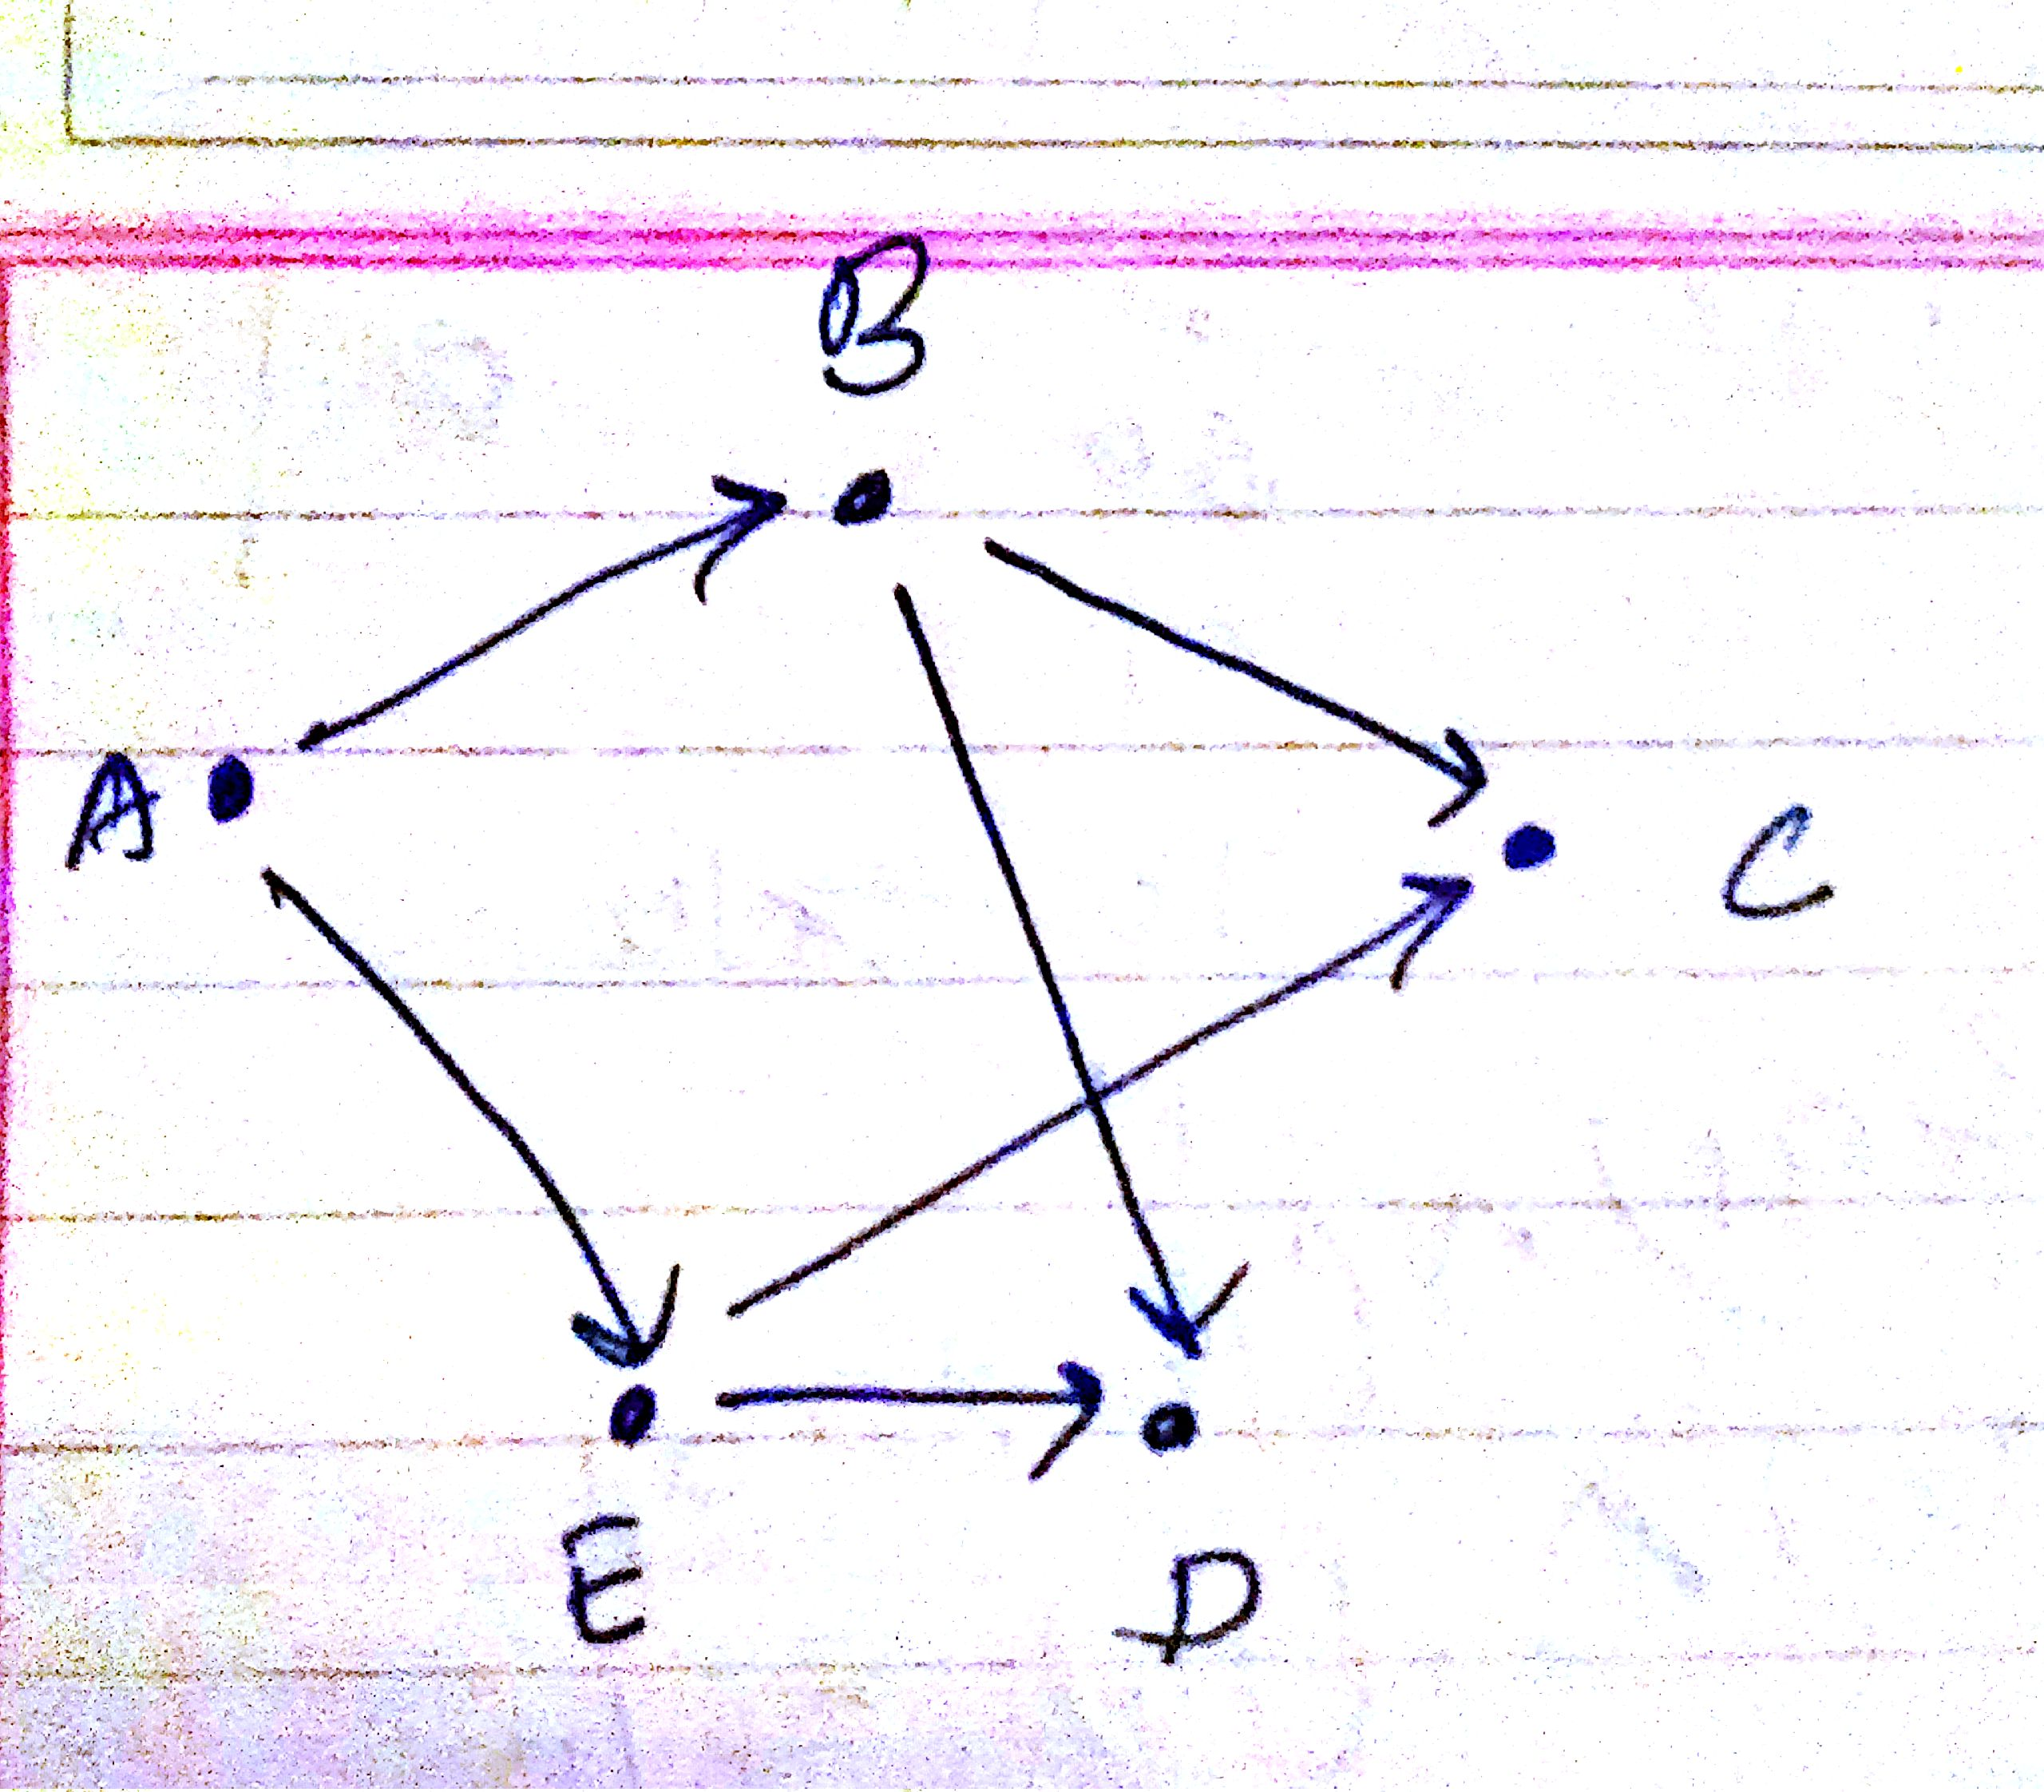
\includegraphics[width=100mm]{image.JPG}
\end{figure}\\
In the figure above, we assume that all edges have the same weight equal to 1. If A be our source vertex, let the set of edges for shortest path to each vertex be E': (A,B),(B,D),(A,E),(C,E). However, if we use BFS, we can never produce these set of paths. Lets say we move to B first. In that case, the set of edges defining shortest paths to each vertex V will be (A,B),(A,E),(B,C),(B,D). Similarly, if we start from E, the set of edges will be (A,E),(A,B),(E,C),(E,D). The set of edges defined by E' can never be produced.\\\\\\
\textbf{Exercise 22.2-7}\\
We can solve this by visualizing the wrestlers and their rivalry as an undirected graph, with wrestlers as nodes and edges as rivalries between any two wrestlers. So, starting from any wrestler s and designating it as heels, if we perform a BFS and designating nodes first as babyfaces and then as heels in alternate cycles, we can achieve such a classification. If ever we come across a node where we are trying to name it as a heel but it has already been named as a babyface or vice versa, then such a classification is not possible. Following is the algorithm. Here instead of color, we store the designation of each wrestler and use the same to identify whether the node has been visited or not.\\\\
We iterate over all the vertices of the graph, to make sure that all vertices are named. On each vertex, we first assign an arbitrary classification and then move into its adjacent vertices alternatively naming them as babyface and heels at each level.\\\\
We maintain a variable to store what should be the designation of each node in every cycle which has to be the opposite of the designation of the node whose edges are being looked at. If the designation of a node was empty, we set its value and enqueue the node. If it is already set and is equal to the value we are trying to set, then it means that this node has already been visited. If in case the value is already set and is different from what we are trying to save then its not possible to achieve a classification and we exit.\\\\
classifyWrestlers(G)
\begin{enumerate}
\item for each vertex u $\epsilon$ G.V - \{s\}
\item \tab{u.designation= null}
\item for(node n in V)
\item \tab{if(u.designation == null)}
\item \tab{\tab{BFS(G, n)}}
\end{enumerate}
BFS(G, s)
\begin{enumerate}
\item s.designation = "heel"
\item queue Q
\item ENQUEUE(Q, s)
\item boolean isPossible = true
\item while (Q not empty \&\& isPossible)
\item \tab{u = DEQUEUE(Q)}
\item \tab{\tab{if (u.designation == "babyface")}}
\item \tab{\tab{\tab{designation = "heel"}}}
\item \tab{\tab{else}}
\item \tab{\tab{\tab{designation = "babyface"}}}
\item \tab{for each v $\epsilon$ G.Adj[u]}
\item \tab{\tab{if (v.designation ==null)}}
\item \tab{\tab{\tab{v.designation = designation}}}
\item \tab{\tab{\tab{ENQUEUE(Q, v)}}}
\item \tab{\tab{else if (v.designation != designation)}}
\item \tab{\tab{\tab{isPossible = false}}}
\item \tab{\tab{\tab{break}}}
\item return isPossible
\end{enumerate}
\newpage
\section{Problem 2}
\textbf{Exercise 22.3-5 a.}\\
A tree edge or forward edge (u,v) means that in the sequence of DFS the node u is visited first, and then while covering the depth of connected nodes of u, v is visited.\\
Since, u is visited before v, we have: $$d[u] < d[v].$$
Also since, v is visited while covering connected nodes of u: $$f[v] < f[u]$$
Since finish times are always greater than starting times: $$ d[u] <  d[v] < f[v] < f[u]$$
\textbf{Exercise 22.3-5 b.}\\
A back edge (u, v) means that u is a descendant of v in the execution of our DFS. That is u is encountered while covering the connected nodes from v. Hence, the same relationship as proved in a holds with u and v reversed. Hence: $$ d[v] <  d[u] < f[u] < f[v]$$
\textbf{Exercise 22.3-5 b.}\\
A cross edge means u and v exist in different trees in the execution of our DFS. During the execution of 1st tree v is encountered but there was no edge connecting the first tree to u. Then during the execution of another tree u is encoutered. Since, v has already been covered, both d[v] and f[v] will be smaller than d[u] and f[u]. Hence:
$$d[v] < f[v] < d[u] < f[u]$$\\
\textbf{Exercise 22.3-11}\\
\begin{figure}[ht!]
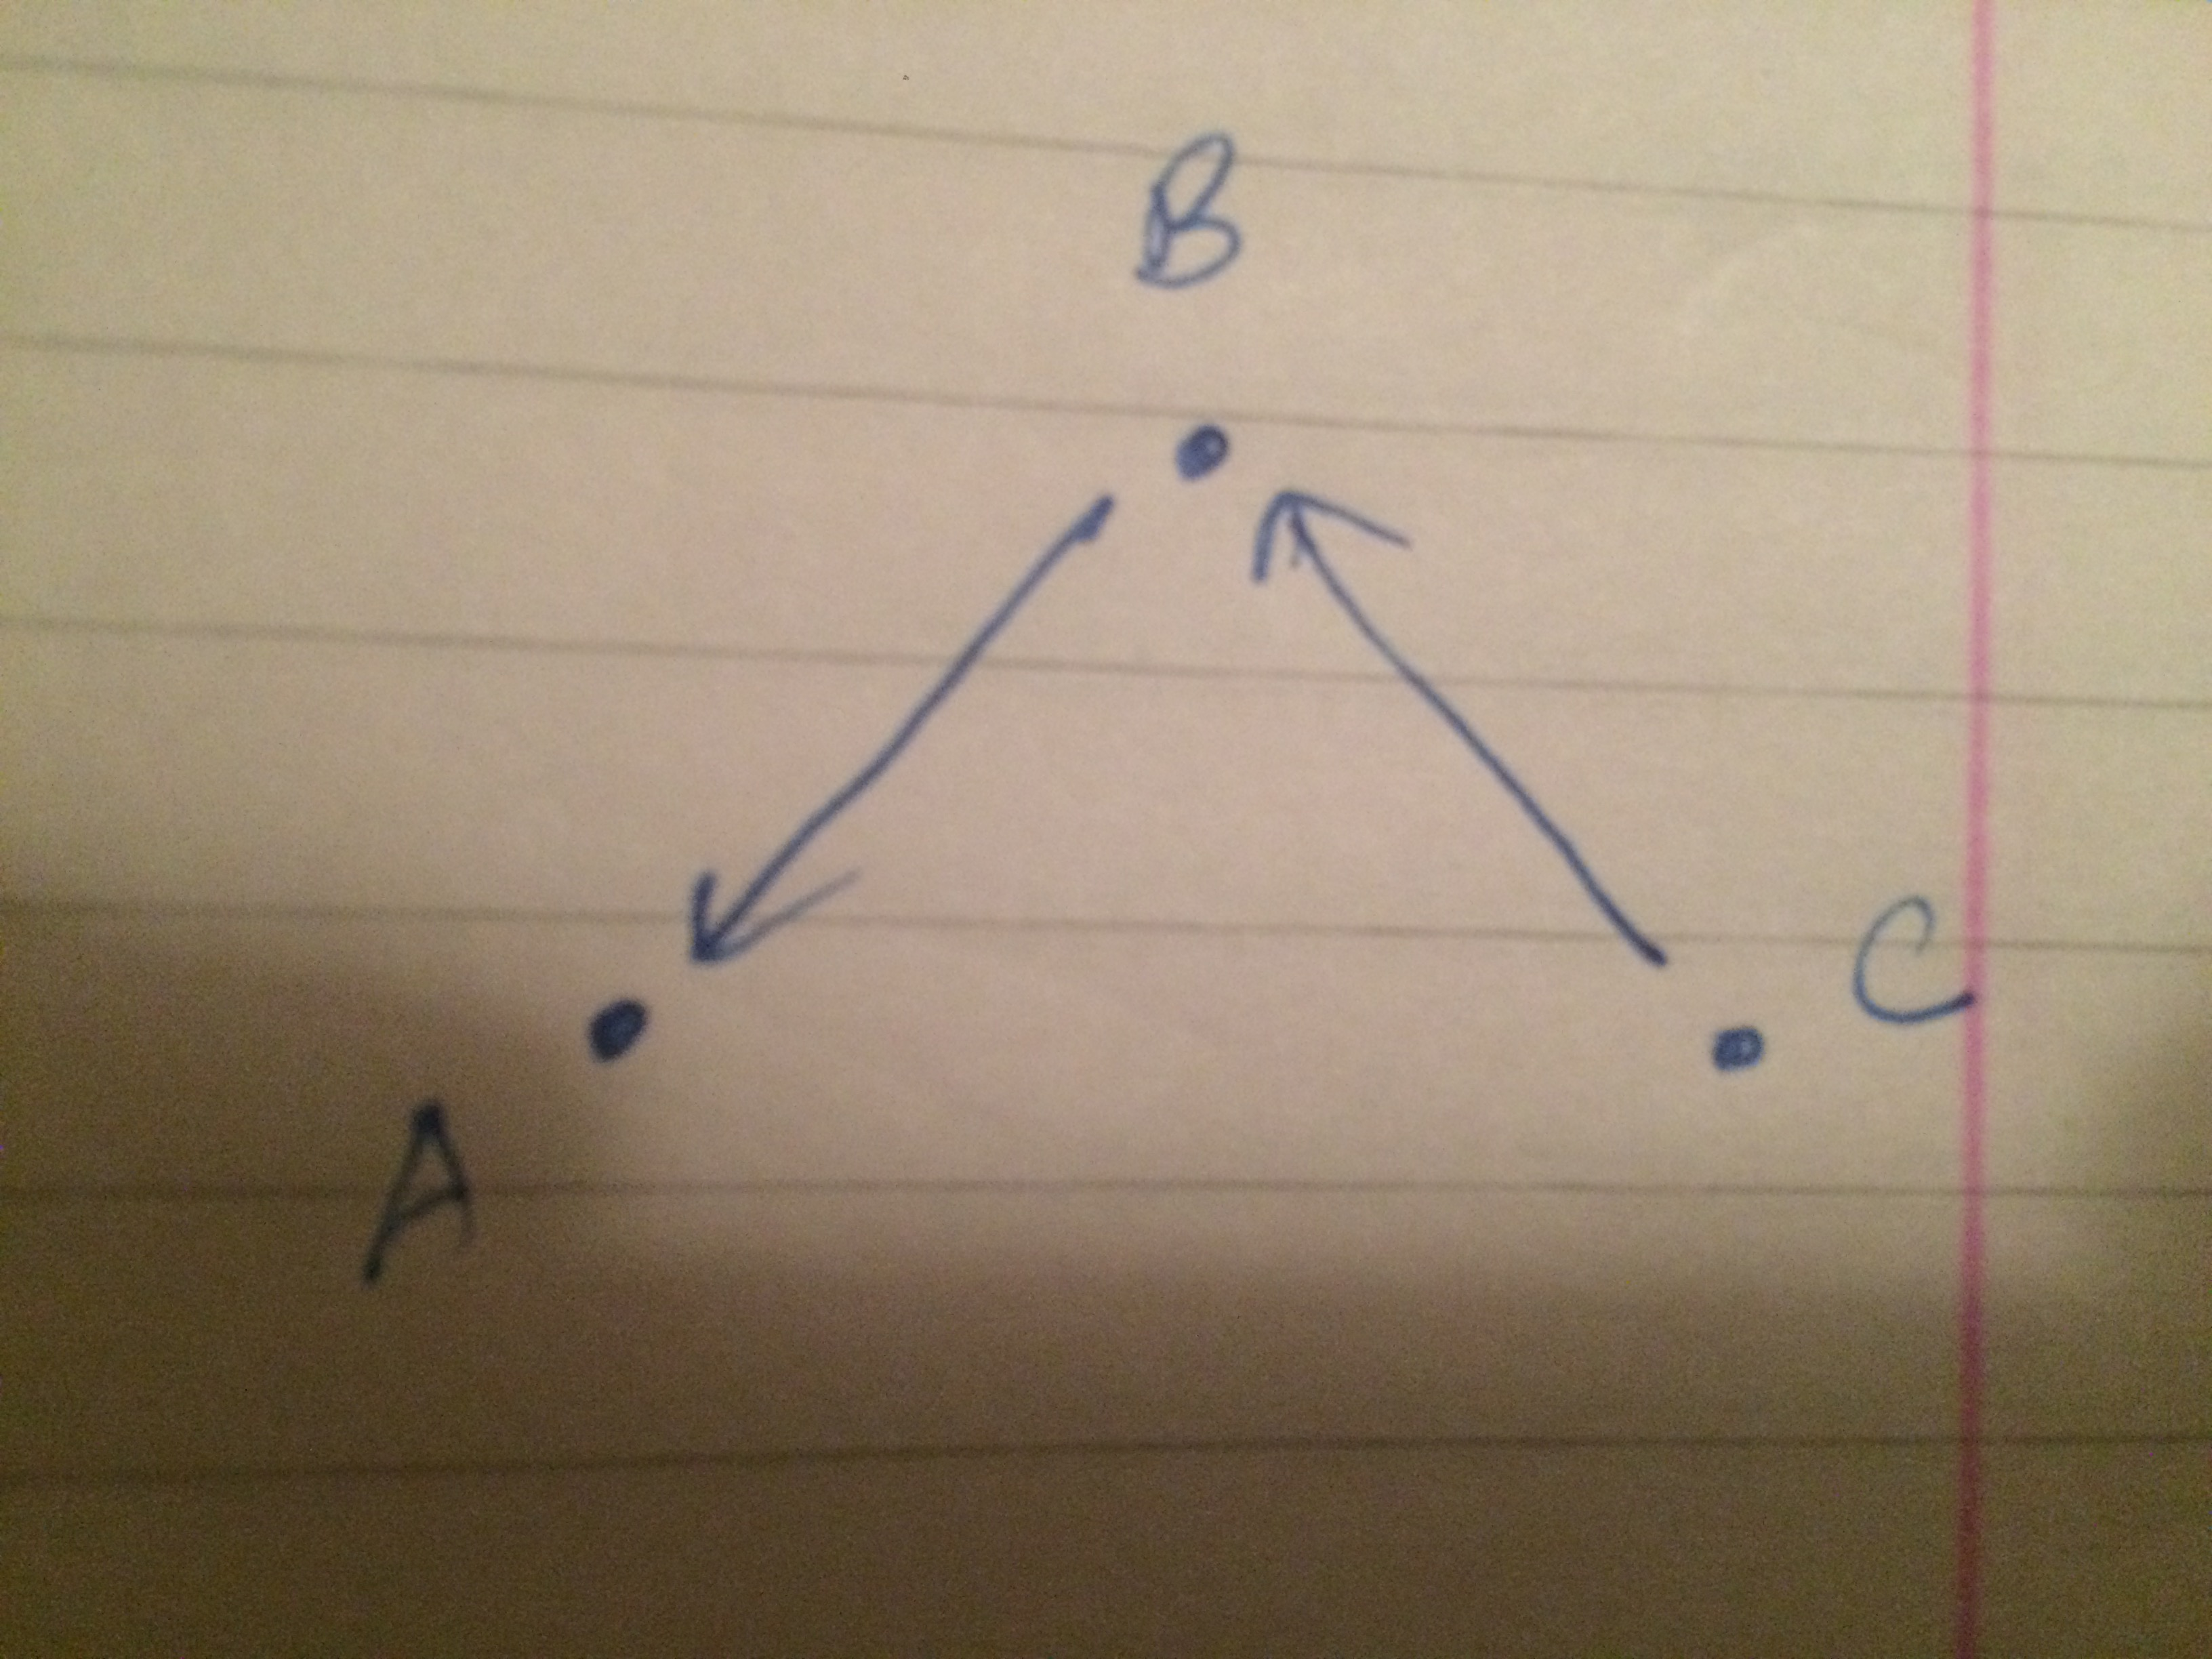
\includegraphics[width=100mm]{IMG_2508.JPG}
\end{figure}\\
The graph shown above has vertices (A, B, C) and edges (B,A) and (C,B). The vertex B has both incoming and outgoing edges. However, if we start the execution of DFS from A and then move in the order to B and then to C, we will have three different subtrees of A, B and C alone. B having both incoming and outgoing edges will still end up in its depth first tree alone.
\newpage
\section{Problem 3}
\textbf{Problem 23-4}\\\\
\textbf{MAYBE-MST-A} removes edges in non increasing order, provided that the graph stays connected even after removing the edge. Since, the edges are being removed in decreasing order of weights, the MST is guaranteed to have all the light edges. Also, since at every step we ensure that the graph is connected, the resulting tree T is the MST of the graph G.\\\\
The most efficient implementation can be using adjacency lists. The sorting of edges can be achieved in O(Elog E) using merge sort. To check whether T-{e} is connected or not we can perform a BFS or DFS which will take O(V+E) time. Since, BFS/DFS is run for each edge, the total time complexity is given by: $$O(E\log E) + O(E(E+V)) = O(E^2)$$\\
\textbf{MAYBE-MST-B} adds edges randomly as long as the graph does not contain cycles after the addition of the edge. It does not take into account the weight of the edges and hence cannot guarantee light edges at each cut. Hence, MAYBE-MST-B cannot result in a MST.
\begin{figure}[ht!]
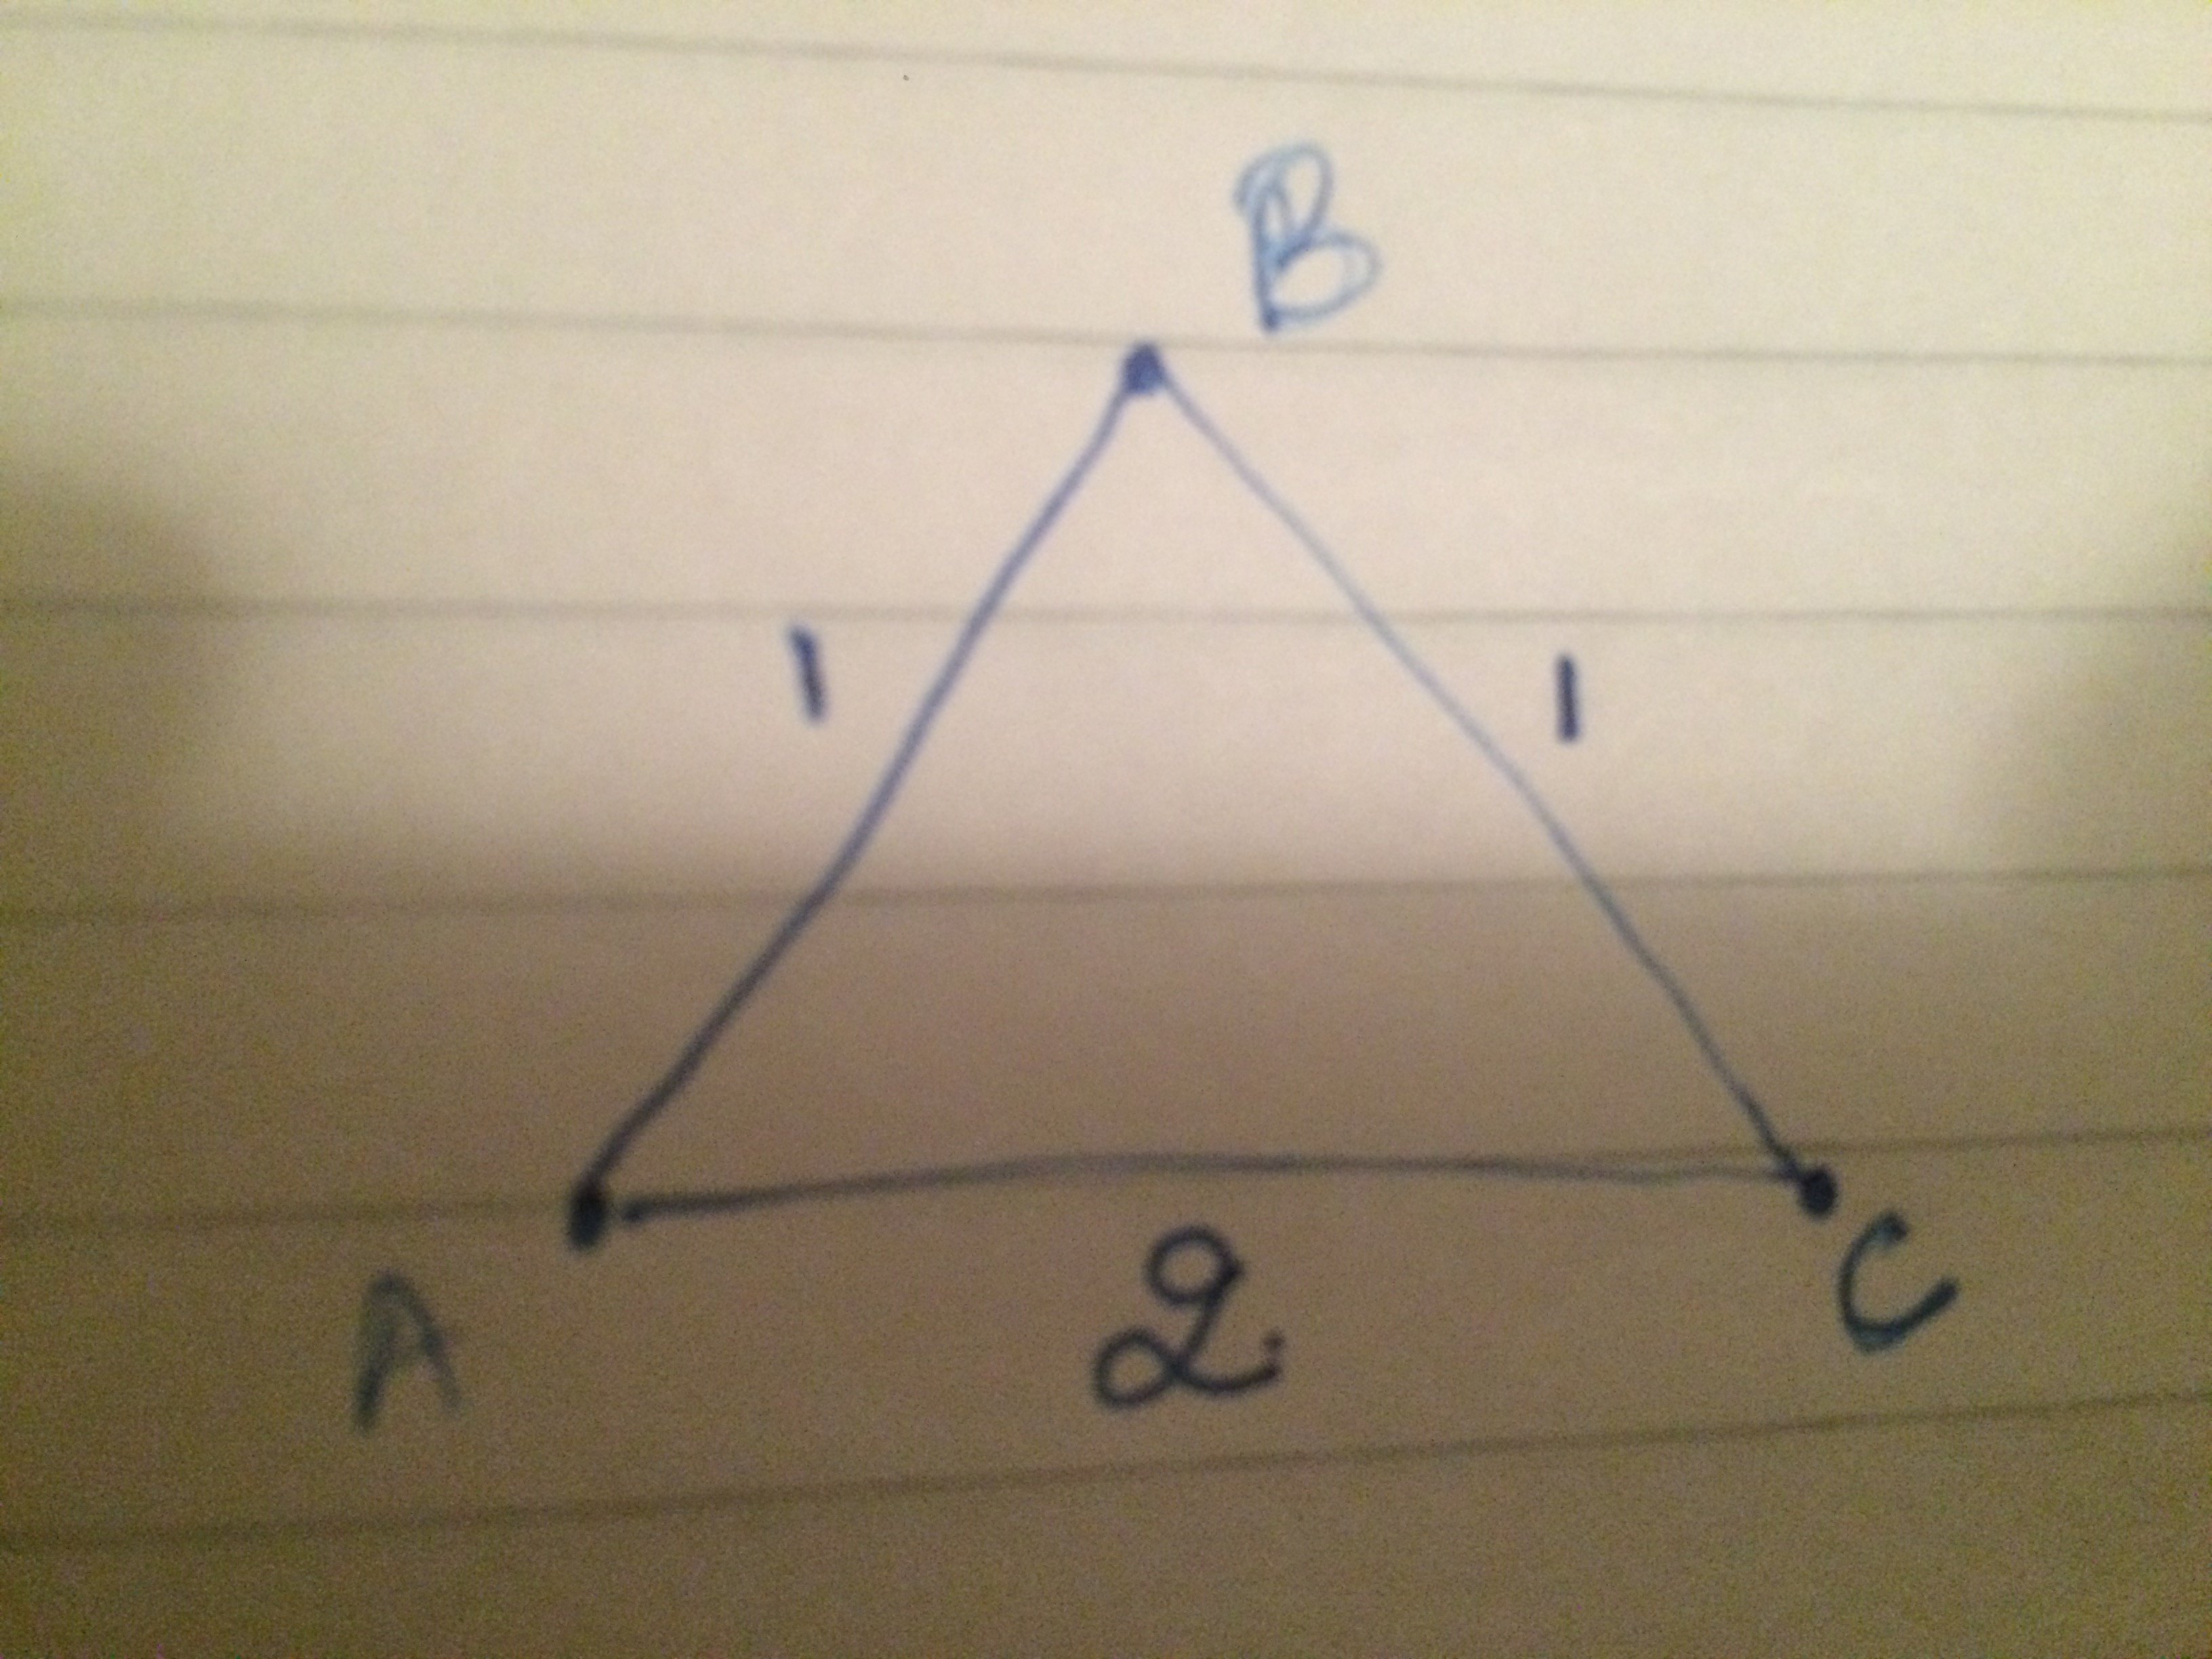
\includegraphics[width=100mm]{IMG_2510.JPG}
\end{figure}\\
A simple example is shown in the figure above. The MST will always contain the edges (A,B) and (B,C). However, since the addition of edges is arbitrary, we could end up with T as either (A,B),(A,C) or as (B,C),(A,C).\\\\
This algorithm is similar to Kruskal's algorithm. We check that T $\cup$ \{e\} has no cycles by FIND-SET(u) $\neq$ FIND-SET(v). Also, mergin e into T happens through the UNION(u) operation. Thus, the complexity is the same as Kruskal's given by $O(E\log \ast V)$.\\\\\\
\textbf{MAYBE-MST-C} adds an edges arbitrarily to T and then checks if T has cycles or not. In case a cycle develops inside T, the edge with the maximum weight is removed. Thus, at the end of the algorithm the graph will be connected since it adds all edges to T and then removes an edge only if a cycle develops within the graph. Also, since it always keeps the edge with the minimum weight in case of a cycle, the T will always have the light edge at completion. Hence, this algorithm will result in a MST.\\\\
For the best implementation, we use an adjacency list. The addition of a graph takes O(1) time, since it can be added at the front. To check a cycle we can perform a DFS which will take O(E+V) time, but since, there can be at most 1 cycle at any point, E is always less than or equal to V. Hence, checking a cycle takes O(V) time. Also, removing an edge can be at most O(V) time in the adjacency list. Since, this is repeated for every edge, the time complexity is: $$E(O(1) + O(V) + O(V)) = O(EV)$$
\newpage
\section{Problem 4}
\textbf{Exercise 23.1-6}\\
Lets say we have a graph G = (V, E). When we move across this graph to create a minimum spanning tree, we achieve a cut of the graph and select a light edge crossing the cut. Now we know that we have unique light edges for every cut. So, at every cut, we will select one of these light edges and move forward, until we have our MST. Since, we have unique light edges at every cut and our MST is a combination of these unique light edges, it can be easily said that we will have a unique MST.\\\\
The converse is not true. The simplest example is a graph of three nodes: A, B and C, with edges (C,B) and (B,A) of cost 1. This has graph a unique MST but the cut ({B},{A,C}) has two light edges of the same cost.\\
\begin{figure}[ht!]
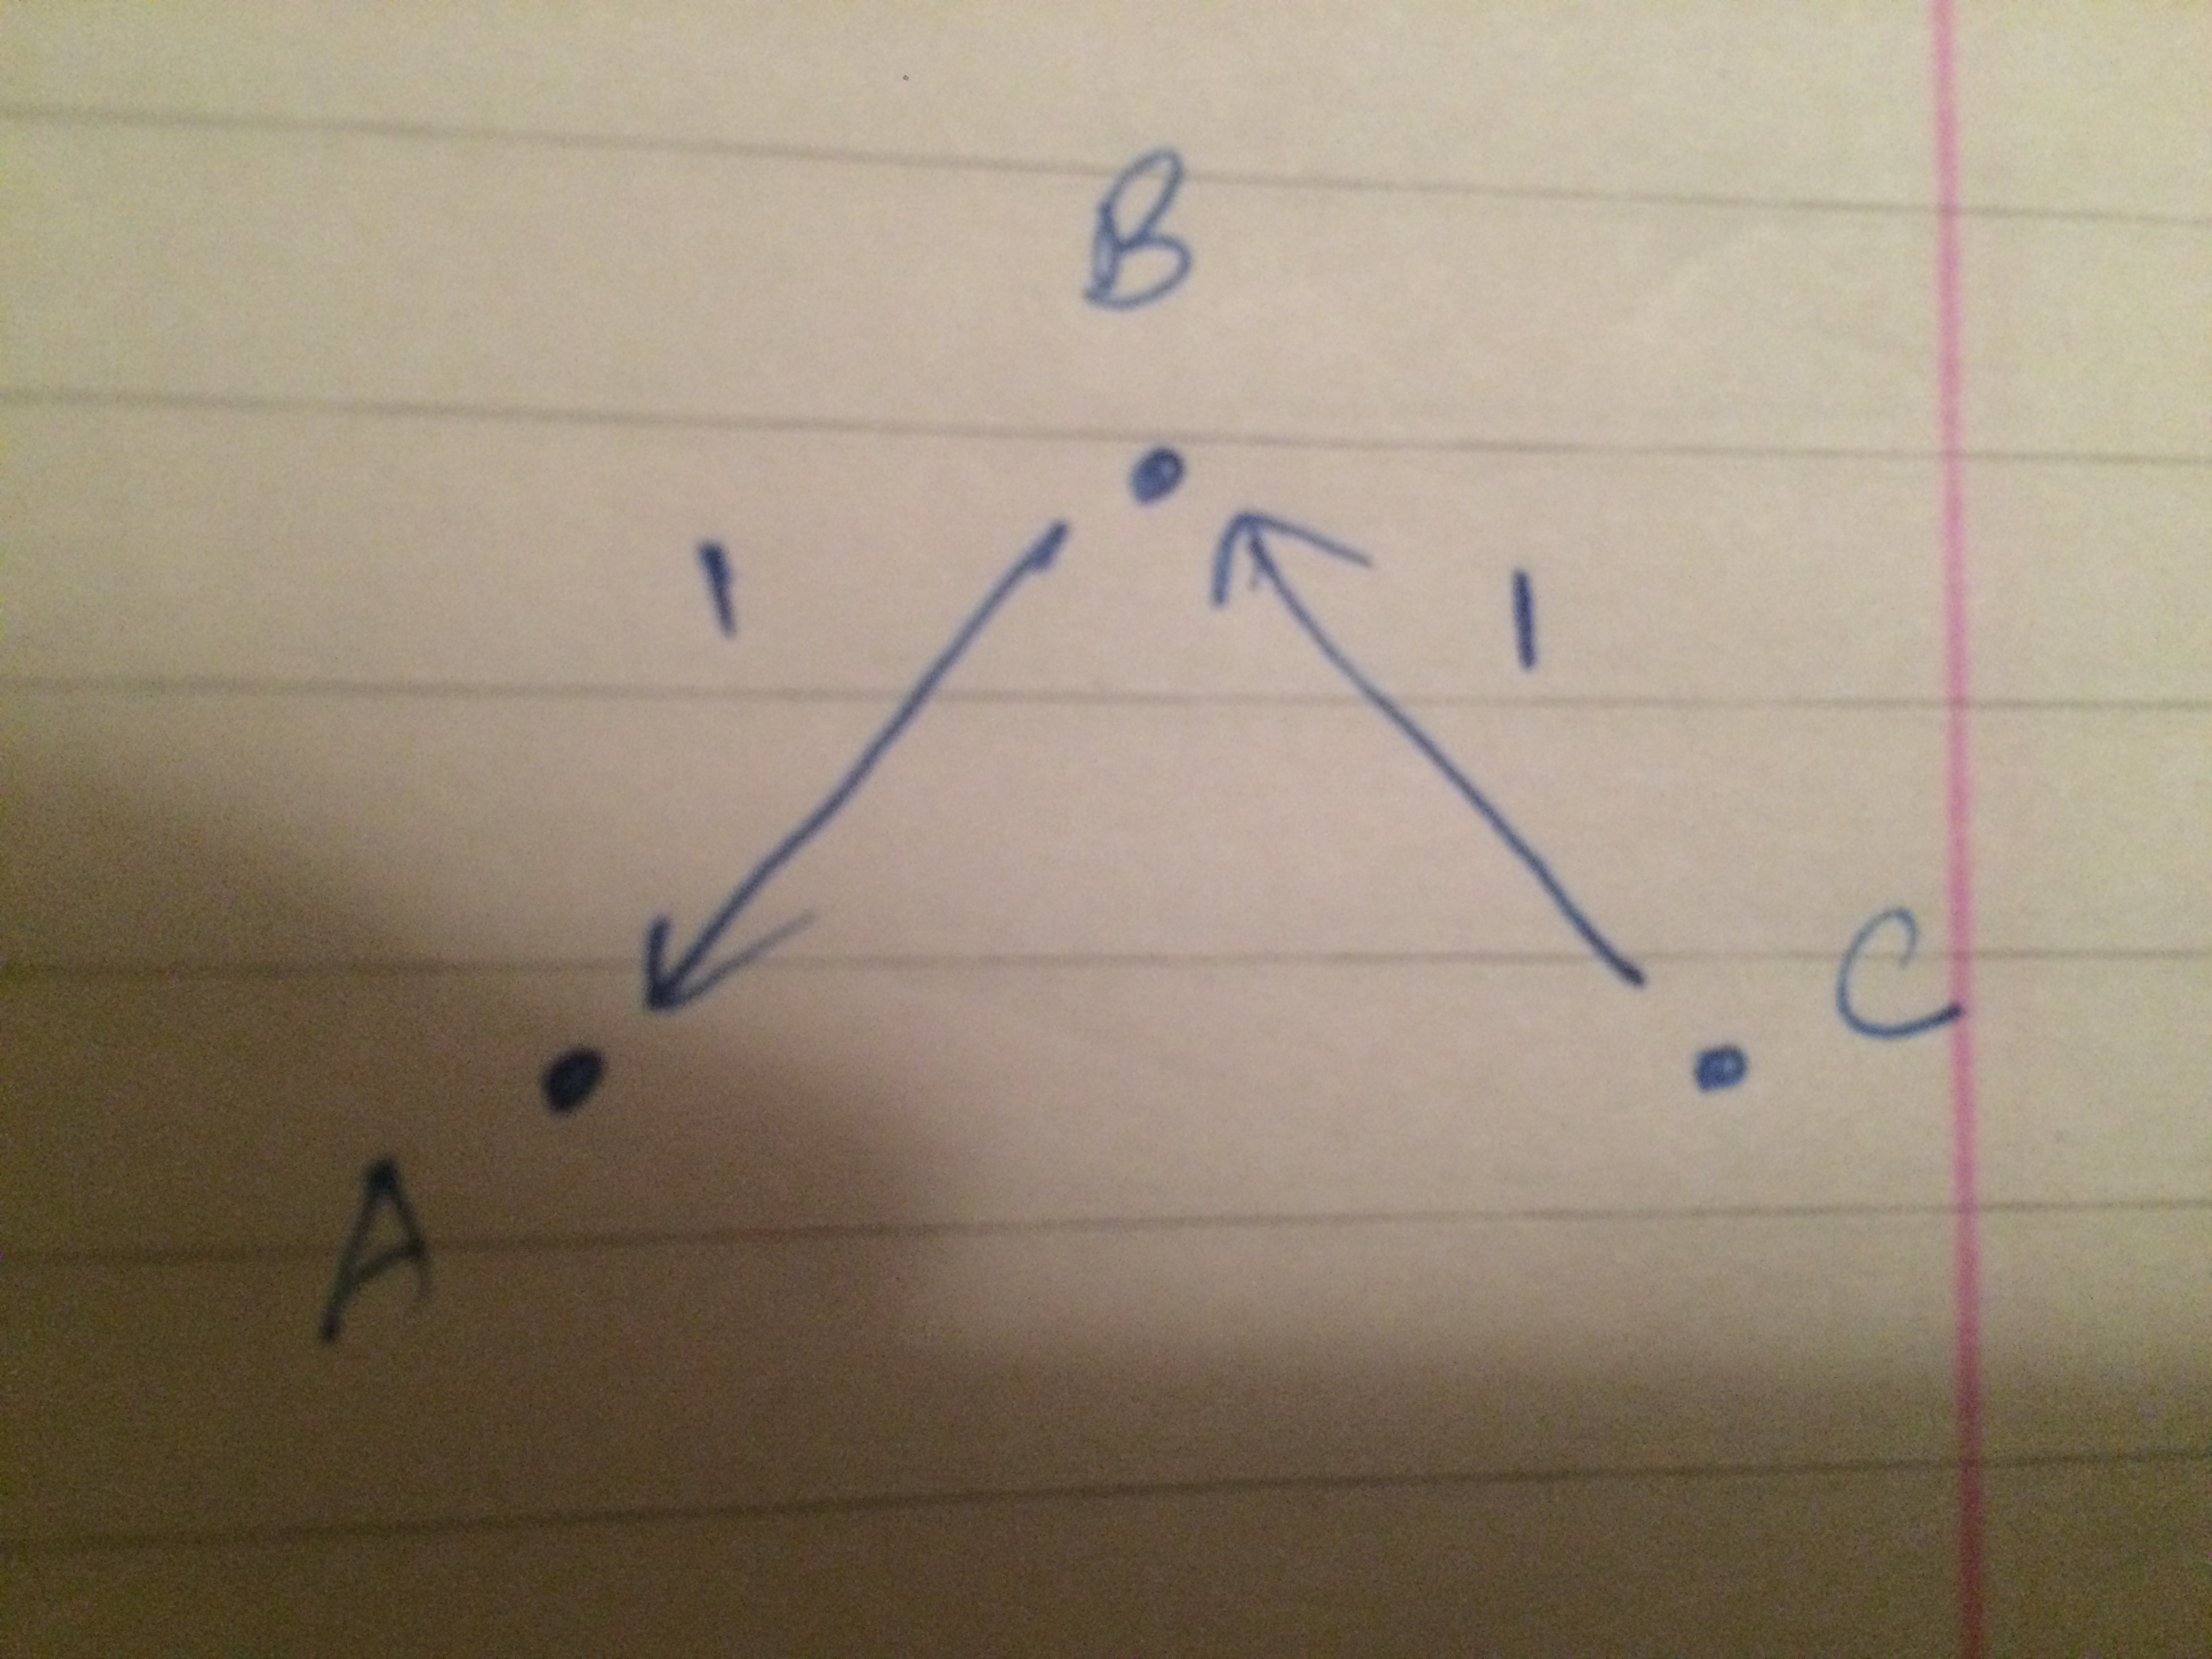
\includegraphics[width=100mm]{IMG_2509.JPG}
\end{figure}\\\\\\\\
\textbf{Exercise 23.1-9}\\
For the graph G = (V,E), we have the MST as T. Now, V' is a subset of V, which defines T' and G' as the subgraph of T and G respectively. Since, T' is the subgraph of T, we know that T' is composed of all the light edges for all possible cuts inside G'. If we know that T' is connected then T' is the MST of G'.
\newpage
\section{Problem 5}
\textbf{Exercise 24.1-5}\\
The question asks us to find for all vertex v $\epsilon$ V, the distances of the vertex u $\epsilon$ V for which v is the nearest neighbour. To achieve this, we can perform a Bellman-Ford like algorithm on a vertex of the above graph. The modification will be in the initialize step which we call at the start of the algorithm and we will have our desired result. Following is the algorithm:\\\\
BELLMAN-FORD(G, w, s)
\begin{enumerate}
\item INITIALIZE-SINGLE-SOURCE (G, s)
\item for i = 1 to $|G.V|$ - 1
\item \tab{for each edge (u, v) $\epsilon$ G.E}
\item \tab{\tab{           RELAX(u, v, w)}}
\item for each edge (u, v) $\epsilon$ G.E
\item \tab{      if v.d $>$ u.d + w(u, v)}
\item \tab{\tab{           return FALSE}}
\item return TRUE\\
\end{enumerate}
INITIALIZE-SINGLE-SOURCE (G, s)
\begin{enumerate}
\item for each vertex v $\epsilon$ G.V
\item \tab{v.d = $\inf$} 
\item \tab{v.$\pi$ = NIL}
\item for each edge (u, v) $\epsilon$ G.E
\item \tab{if v.d $>$ w(u,v)}
\item \tab{\tab{v.d = w(u,v)}}
\end{enumerate}
Since, we modified the INITIALIZE-SINGLE-SOURCE function to initialize v.d as the weight of the minimum weight edge to v from some vertex u, and during RELAX, we update v.d as the minimum distance to v from a vertex u, as the algorithm continues, v.d will be updated with the minimum distances from all vertices.\\\\\\
\textbf{Exercise 24.5-5}\\
An example of such a graph is shown in the image below. There are two shortest paths from A to B: $A->B$ and $A->D->B$, both of weights 5. Similarly, there are two paths from A to C and A to D. Now, if we name $v.\pi$ to as a parent on any of the shortest paths, we can have a situation where:\\
$B.\pi = D$
$C.\pi = B$
$D.\pi = C$
Thus, we see that a cycle has been generated within B,C,D if such a way is used.
\newpage
\begin{figure}[ht!]
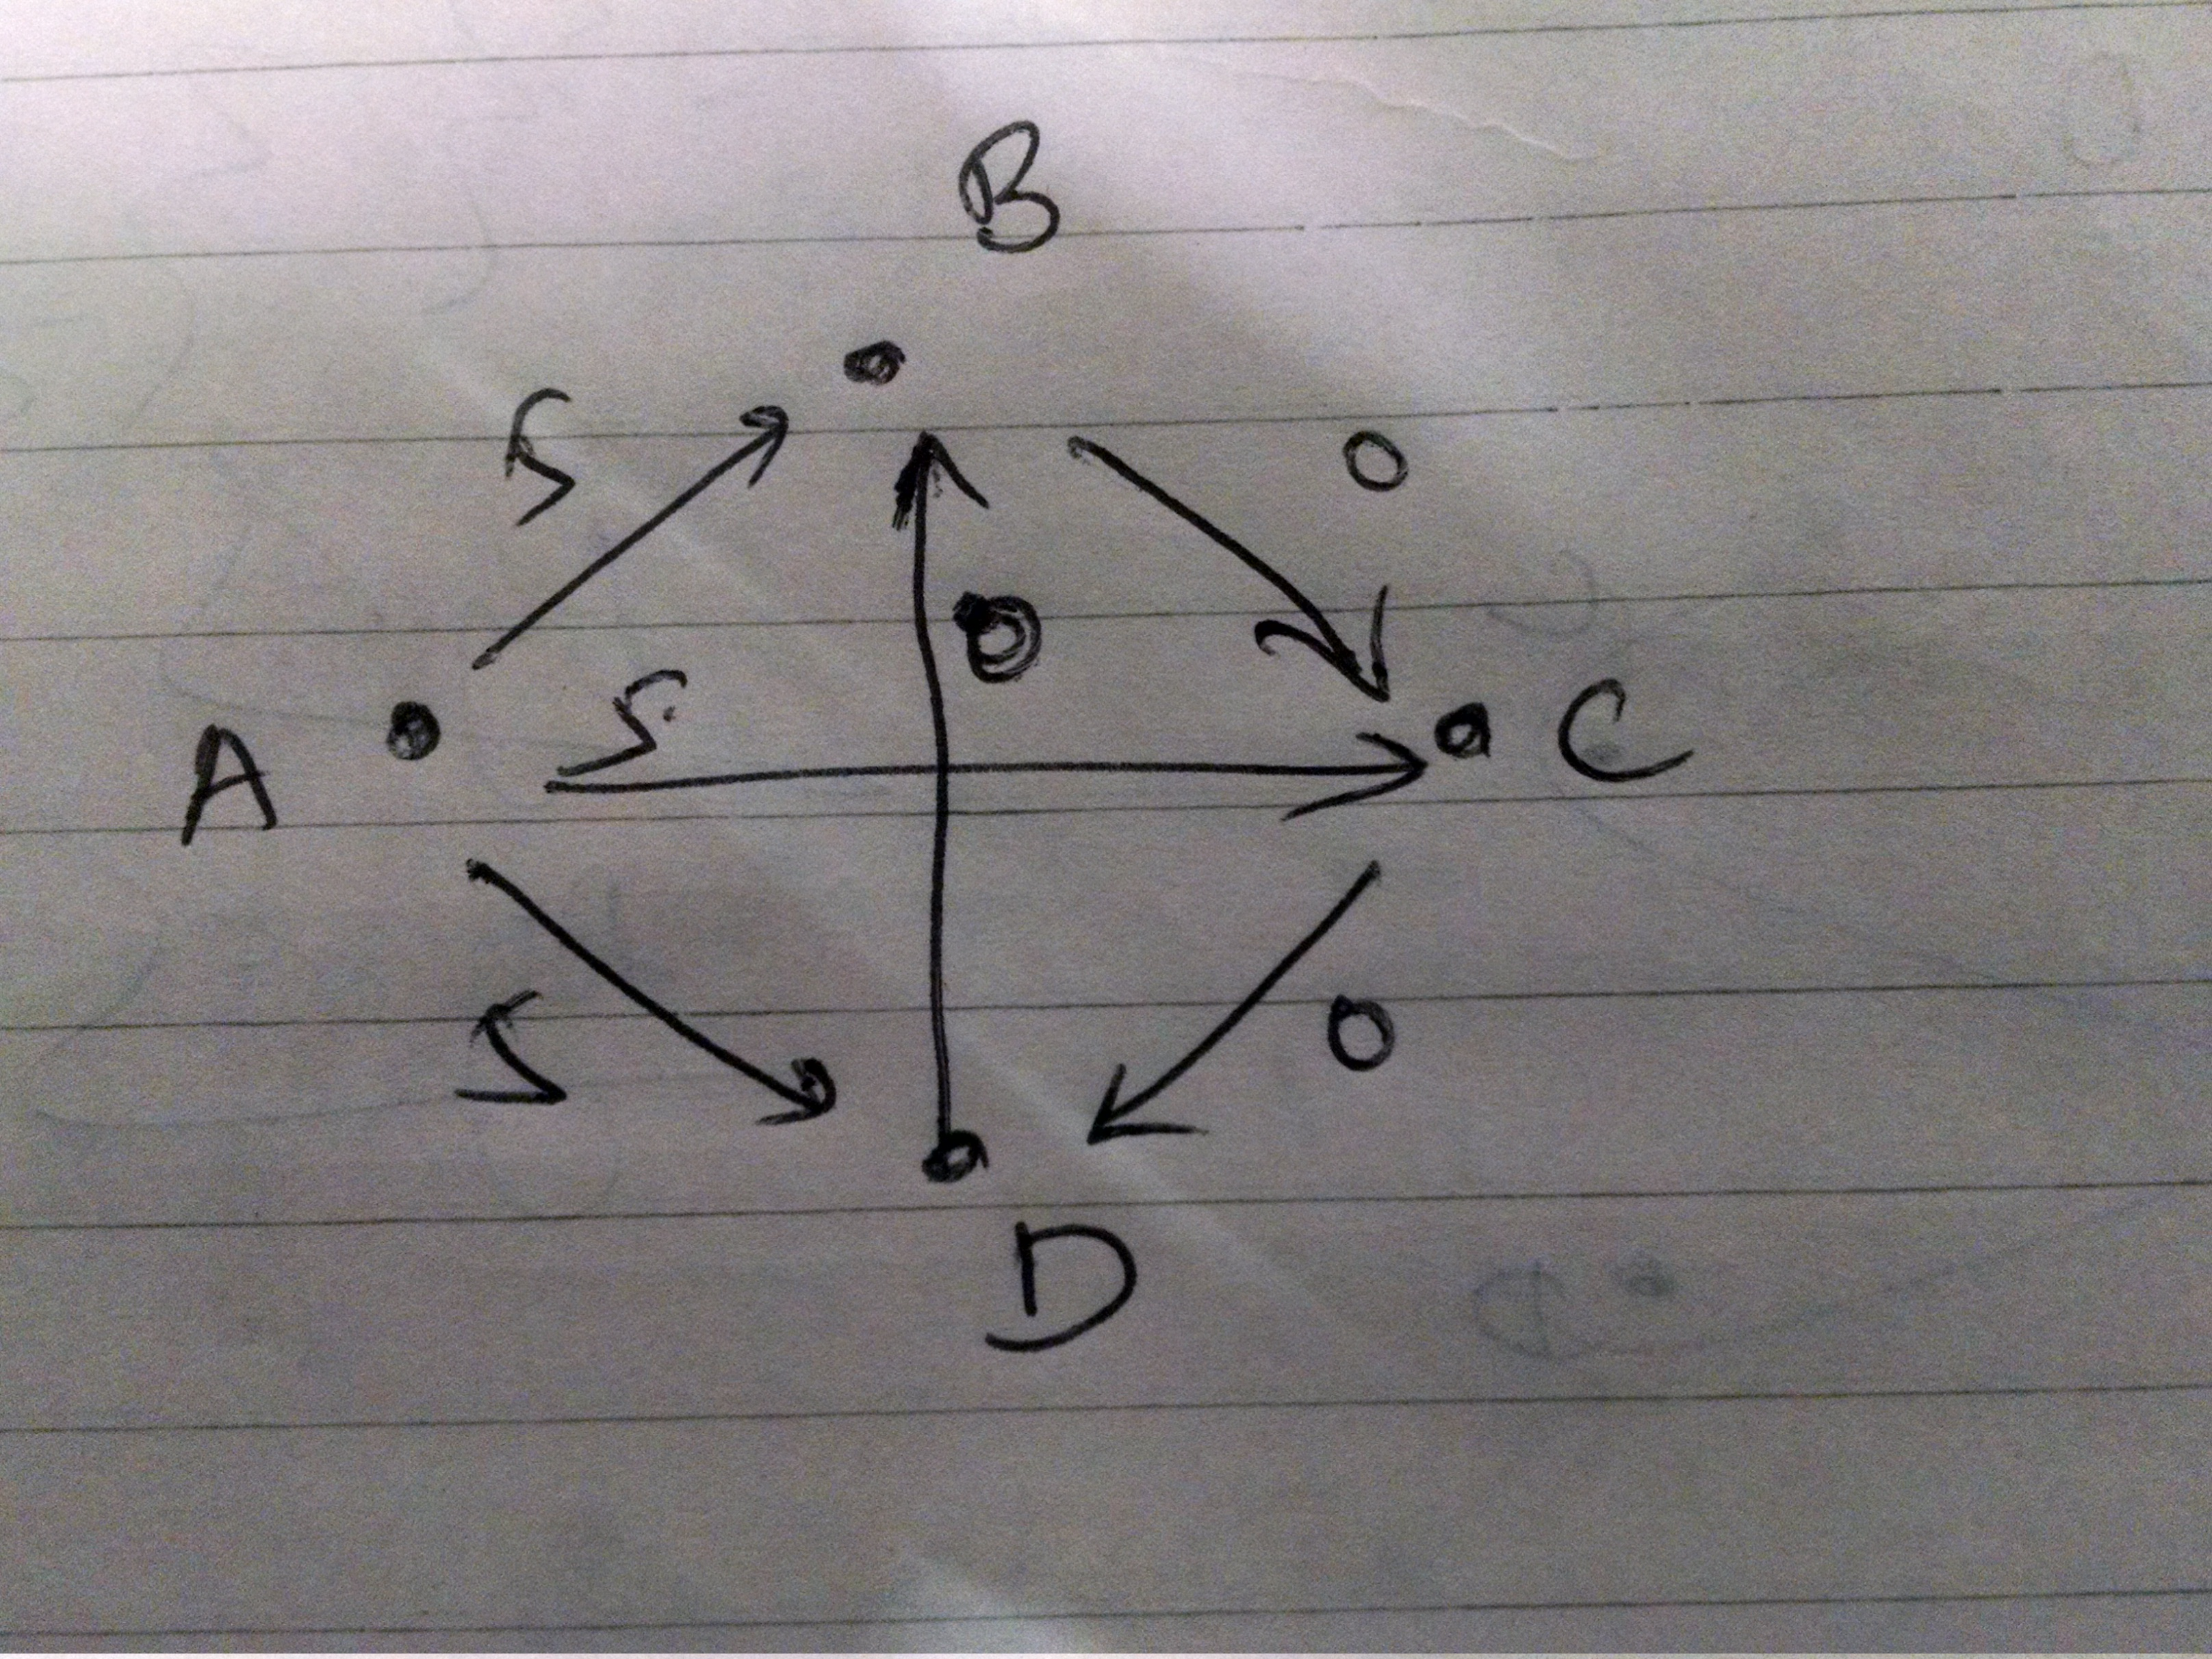
\includegraphics[width=100mm]{IMG_2511.JPG}\\
\end{figure}
\newpage
\section{Problem 6}
\textbf{Exercise 24-4 a.}\\
Since we know that all weights are positive, we can use Dijkstra's algorithm to find the shortest paths from the source vertex s to all vertices v. However, we also know that all our weights are bounded by $|E|$. Hence, we do not need to use a min-heap or a priority queue for the vertices. We can do better by using an array of size $|E|+1$ of linked lists, so that the linked list at position i in the array holds all vertices at distance i from the source vertex.\\\\
Lets say we denote our array with Q. Initially, we add all elements to the list Q($|E|+1$), so that all elements are in Q. When, the key v.d of a node decreases we simply add the element to the front of the list Q[i]. Thus this operation can take place in O(E) time. During EXTRACT-MIN, we simply remove the topmost element of the list Q[i]. We store the position i of the linked list from where the last EXTRACT-MIN element was performed. In the next iteration, we can start scanning for the next EXTRACT-MIN from this i. We can do this, since the minimum distance always increases as we traverse the graph and we do not need to go back. In this way, we can perform our $|V|$ EXTRACT-MIN in O(E) time.
Thus the time complexity is $E \times O(1) + O(E) = O(E)$.\\\\\\
\textbf{Exercise 24-4 b.}\\
We can use the part a. to prove this. Since, $w_1$ uses only the first significant bit of the weight function the maximum value of the weight of each edge can be 1. Hence, the maximum value of $\delta_1(s, v)$ can be V-1(when all the edges are included in the shortest path to a node). Since we have an upper limit on our weights, we can use the algorithm stated in part a to compute $\delta_1$.\\\\\\
\textbf{Exercise 24-4 c.}\\
We know that, $w_i = \lfloor w(u,v)/2^{k-i} \rfloor$. Hence, it can be seen that $w_i = 2w_{i-1}$ + b, where b is the last bit in $w_i$. If b is 0, $w_i = 2w_{i-1}$, whereas if b=1, $w_i = 2w_{i-1}$ + 1.\\\\
Now as stated in part b, $\delta_i$, is the minimum of the sum of weights from source s to v across various paths. Since, the weights on each edge at least doubles from $w_{i-1}$ to $w_i$, $\delta_i$ is at least $2\times \delta_{i-1}$. Stated numerically, $$\delta_i \geq 2 \times \delta_{i-1}$$.
The upper limit can be achieved from the fact that the weight of each edge can be at most $2\times \delta_{i-1} +1$. Now, the longest delta can be composed of V-1 vertices and hence, $$\delta_i \leq 2 \times \delta_{i-1} + V - 1$$\\\\.\textbf{Exercise 24-4 d.}\\
We know that, $$\delta_{i-1}(s,v) \leq \delta_{i-1}(s, u) + w(u,v)$$
$$2\delta_{i-1}(s,v) \leq 2\delta_{i-1}(s, u) + 2w_{i-1}(u,v)$$
$$2w_{i-1}(u,v) + 2\delta_{i-1}(s, u) -2\delta_{i-1}(s,v) \geq 0$$
$$w_{i}(u,v) + 2\delta_{i-1}(s, u) -2\delta_{i-1}(s,v) \geq 0$$
$$\widehat{w_{i}}(u,v) \geq 0$$
\textbf{Exercise 24-4 e.}\\
From above we know that $$\widehat{w_i}(u,v) = w_i(u,v) + 2\delta_{i-1}(s,u) - 2\delta_{i-1}(s, v)$$
Similarly, $$\widehat{w_i}(t,u) = w_i(t, u) + 2\delta_{i-1}(s,t) - 2\delta_{i-1}(s, u)$$
Adding the above two, we get:
$$\widehat{w_i}(u,v)+\widehat{w_i}(t,u)  = w_i(u,v) + w_i(t,u) + 2\delta_{i-1}(s,t) - 2\delta_{i-1}(s, v)$$
We see that for sum of reweighted value of two paths contains only the terms $2\delta_{i-1}(s,t)$ and $2\delta_{i-1}(s, v)$ and cancels out for the intermediate u.
We know that $\widehat{\delta_i}(u,v)$ is some of such weight functions across the minimum cost path. Hence, the sum will only consist of delta for (s,s) and (s,v). All the intermediate points will get cancelled:
$$\widehat{\delta_i}(u,v) = \Sigma \widehat{w_i}(e) = \Sigma w_i(e) + 2\delta_{i-1}(s,s) - 2\delta_{i-1}(s,v)$$
$$\widehat{\delta_i}(u,v) = \Sigma w_i(e) - 2\delta_{i-1}(s,v)$$
$$\widehat{\delta_i}(u,v) = \delta_i (s,v) - 2\delta_{i-1}(s,v)$$
$$\delta_i (s,v) = \widehat{\delta_i}(u,v) + 2\delta_{i-1}(s,v)$$\\\\\\
\textbf{Exercise 24-4 f.}\\
We can compute $\delta_i(s, v)$ from $\delta_{i−1}(s, v)$ for all v $\epsilon$ V in O(E) time by using the following steps:
\begin{enumerate}
\item We compute the quantities $\widehat{w_i}(u, v)$ by the formula shown in part (d). This takes O(E) time.
\item Using part (e), $\delta_i(s, v) \leq |E|$, so we can compute all $\widehat{\delta_i}$(s, v) in O(E) time using part (a).
\item Using 2. $\widehat{\delta_i}(s, v)$ from $\delta_i$(s, v) and $\delta_{i−1}(s, v)$ can be calculated in O(V) time.
\end{enumerate}
Starting from $\delta_1(s,v)$, computed in part 2, we can repeat the above steps for each successive bit to k times to arrive at our final $\delta(s,v)$ result. Since, each step above takes O(E) time, the total algorithm can be performed in O(kE) = O(E logW).
\end{document}